Once our data is in functional form, we may encounter an interesting phenomenon
that creates problems in FDA. In many situations, functional observations have
similar shapes, but they are in some way misaligned. This variability will
interfere with further analysis, and therefore, a registration of our data will
be necessary in order to eliminate and quantify its variation.

\begin{figure}[Male growth rate]{FIG:BERKELEY}{Male growth rate}
	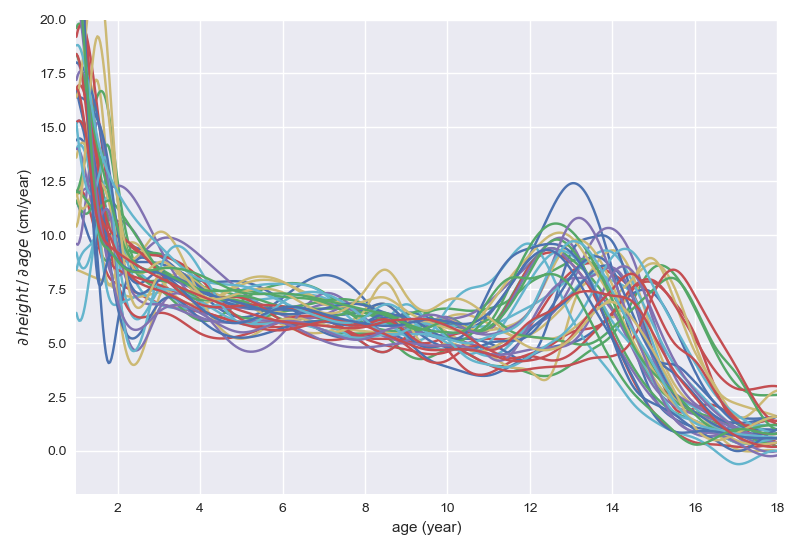
\includegraphics[width=11cm]{berkeley-males}
\end{figure}

The Berkeley Growth Study\cite{berkeley}, performed in 1954, recorded the heights of 54
girls and 39 boys between the ages of 1 and 18 years. In the figure
\ref{FIG:BERKELEY} it is shown the velocity growth curves of the boys. Every curve shows a main stage of growth corresponding with the puberty;
however, these stages are not aligned due to hormonal and other
physiological factors in the growth. The rigid metric of physical time may not
be directly relevant to the internal dynamics of our problem, so it may be
convenient to make a transformation of the time scale to adapt it to the nature
of our data. In the registration of the data, or alignment, this type of
variability is analyzed, quantified and separated.



The variability of the data can be decomposed into two sources; the first one
comes from the random curve-to-curve variation\cite{Kokoszka2017}, this is called
\textbf{amplitude variation}. In the figure \ref{SBFIG:AMPLITUDE} it is shown a
set of curves whose variability proceeds exclusively from the amplitude. The
second type proceeds from misalignments of the curves with respect to the
domain; this is called \textbf{phase variation}. In the figure
\ref{SBFIG:PHASE} it is shown a set of curves whose variation is completely due
to the phase; this source of variability is the one that will be dealt with in
the registration process.

\begin{figure}[Amplitude and phase variability]{FIG:AMPPHA}{Amplitude and phase variability}
  \subfigure[SBFIG:AMPLITUDE]{Dataset with amplitude variability}{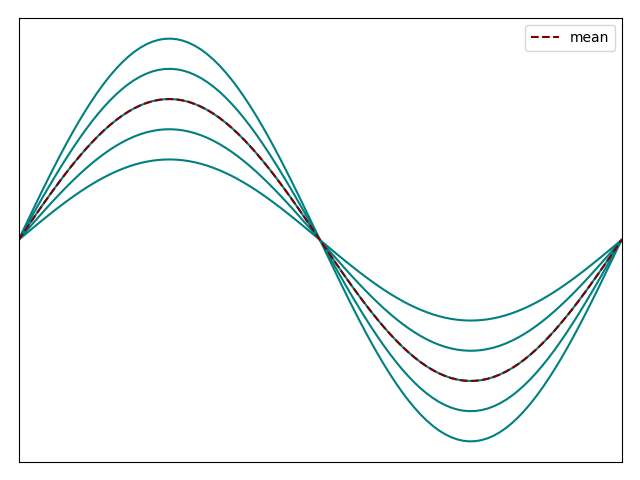
\includegraphics[width=7.5cm]{amplitude-variation}} \quad
  \subfigure[SBFIG:PHASE]{Dataset with phase variability}{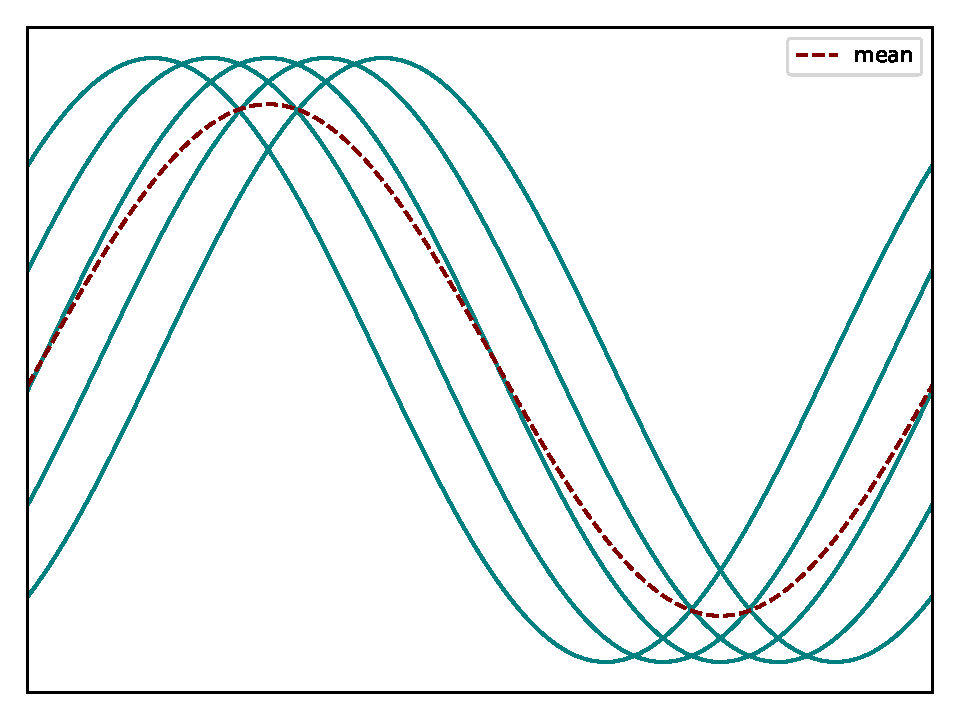
\includegraphics[width=7.5cm]{phase-variation}}
\end{figure}
